\documentclass{standalone}
\usepackage{tikz,pgfplots}
\pgfplotsset{compat=newest}
\begin{document}

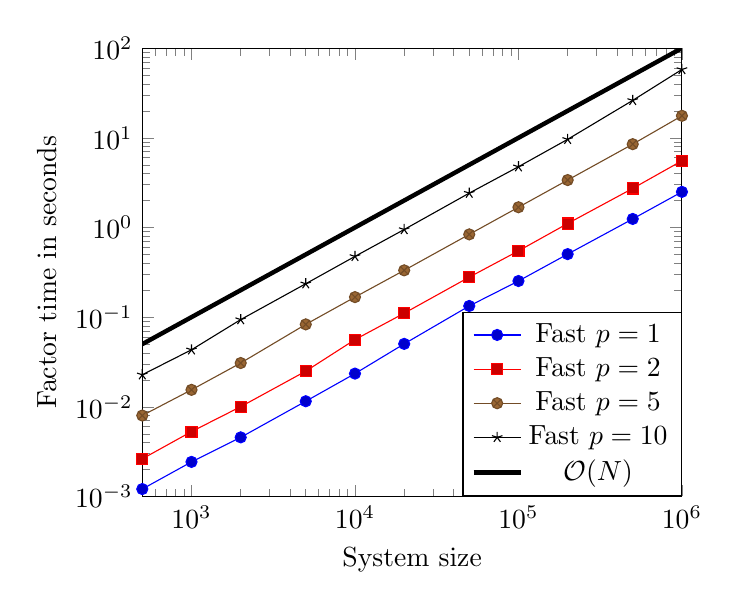
\begin{tikzpicture}
\begin{loglogaxis}[
	xlabel={System size},
	ylabel={Factor time in seconds},
	xmin=500, xmax=1000000,
	ymin=1e-3, ymax=1e2,
	legend style={
  		at={(1.0,0.0)},
		anchor=south east},
]
%Fast m=1
\addplot
coordinates{
(500, 0.00121) (1000, 0.00243) (2000, 0.004564) (5000, 0.011534) (10000, 0.023463) (20000, 0.050336) (50000, 0.13328) (100000, 0.252942) (200000, 0.504634) (500000, 1.24524) (1000000, 2.49585) 
};
\addlegendentry{Fast $p=1$}
%Fast m=2
\addplot
coordinates{
(500, 0.002629) (1000, 0.00529) (2000, 0.010029) (5000, 0.024969) (10000, 0.056163) (20000, 0.110601) (50000, 0.279334) (100000, 0.548) (200000, 1.10696) (500000, 2.7264) (1000000, 5.54856) 
};
\addlegendentry{Fast $p=2$}
%Fast m=5
\addplot
coordinates{
(500, 0.007996) (1000, 0.015466) (2000, 0.030792) (5000, 0.083074) (10000, 0.167298) (20000, 0.332716) (50000, 0.837808) (100000, 1.68176) (200000, 3.37965) (500000, 8.49651) (1000000, 17.5993) 
};
\addlegendentry{Fast $p=5$}
%Fast m=10
\addplot
coordinates{
(500, 0.022781) (1000, 0.043252) (2000, 0.093907) (5000, 0.235806) (10000, 0.47596) (20000, 0.949532) (50000, 2.41607) (100000, 4.76024) (200000, 9.62071) (500000, 26.1528) (1000000, 57.8494)
};
\addlegendentry{Fast $p=10$}
%O(N) scaling
\addplot[ultra thick, no marks]
coordinates{
(500, 0.05) (1000000, 100)
};
\addlegendentry{$\mathcal{O}(N)$}
% %O(N^3) scaling
% \addplot
% coordinates{
% (500, 0.1) (5000, 100)
% };
% \addlegendentry{$\mathcal{O}(N^3)$}
% %Usual
% \addplot
% coordinates{
% (500, 0.012278) (1000, 0.086299) (2000, 0.638305) (5000, 9.42347) (10000, 72.4561)
% };
% \addlegendentry{Usual algorithm}
\end{loglogaxis}
\end{tikzpicture}
\end{document}